%%%%%%%%%%%%%%%%%%%%%%%%%%%%%%%%%%%%%%%%%%%%%%%%%%%%%%%%%%%%%%%%
\section{Proposed Methodology}

In this section I will provide details of how I will address the posed
problems. First, I will present theory of copulas and show how one can use
them to construct \trish{a mixture} model of dependent variables. Second, I
will describe a Monte Carlo method to obtain performance predictions for
the proposed models. Lastly, I will present Bayesian methods of statistical
inference, including hierarchical models, Markov Chain Monte Carlo sampler
and posterior sample diagnostics, model selection, \trish{and} posterior
predictive checks.  \trish{Delete:, broken up into several subsections.}

\subsection{Copula-based modeling of associations}

Development of cognitive process models, \trish{Delete: that describe an
  association structure between component processes involved in a sequence
  of simple decisions}, requires selecting a multivariate distribution for
the covarying parameters. In the context of modeling speeded decisions with
the Ratcliff model, this problem is both underconstrained, given the lack
of information about the association structure, and restricted, because the
parameters \trish{do not have the same scale.} Hence, the method of
construction should allow combining an arbitrary association structure and
arbitrary univariate marginals.

\trish{Insert the beginning of a running example here.  E.g., ``Consider
  [some model or another] with parameters [list them] that explain [some dependent
  variables].''  Explain what you meant above by being underconstrained and
  restricted by pointing to features of the running example.  Then describe
  the association structure (for the parameters?) and provide a segue into
  the next paragraph.}  

The framework of copulas, developed in probability theory over the last 60
years and recently imported for data analysis in a variety of fields, is
well-suited for this problem
\citep{Skl1959,Joe1997,Nel2007,BerWoo2008}. Mathematically, a copula is a
function $C(u_1, u_2, \dots, u_p): [0, 1]^p \mapsto [0, 1]$ that maps a
point $(u_1, u_2, \ldots, u_p)^T$ from a $p$-dimensional unit hypercube to
a point in a unit interval.  Probabilistically, a copula is a probability
distribution on a standard hypercube with continuous, uniformly distributed
univariate marginals $U_i \sim \mathcal{U}(0, 1), i = 1, 2, \dots, p$
\trish{with a specified(?) correlation structure?}. Figure \ref{fig:copula}
shows samples drawn from four copulas with approximately matched level of
dependence including normal, Clayton, Gumbel and Frank.

\begin{figure}
\centering
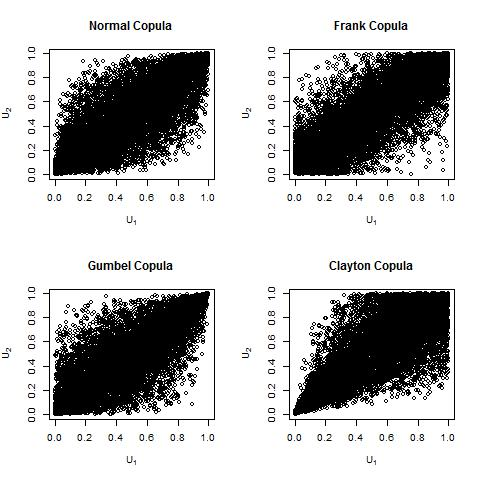
\includegraphics[width=0.9\textwidth]{4_Copulas}
\caption{}
\label{fig:copula}
\end{figure}

\trish{Discuss now the application of copulas, not mathematically, but
  conceptually, to the specifics of your running example.}

The fundamental result that makes copulas important for constructing models
with \trish{Note: ``dependent variables'' is too easy to confuse with
  ``dependent variables.''} correlated parameters \trish{Delete: dependent
  variables} is due to Sklar's \citeyear{Skl1959} two-part representation
theorem:
%
\newtheorem*{Sklar}{Theorem} 
\begin{Sklar} 
Let $F$ be a multivariate distribution with continuous marginal
distributions $F_1, F_2, \dots, F_p$, then there exists a unique
copula $C$ such that 
%
\begin{equation}
\label{eqn:sklar}
F(x_1, x_2, \dots, x_p) = C(F_1(x_1), F_2(x_2),
\dots, F_p(x_p)).
\end{equation}
%
Conversely, given a copula $C$ and marginal univariate distributions $F_1,
F_2, \dots, F_p$, \trish{$F$} is a multivariate distribution.
\end{Sklar}

The forward implication of Sklar's theorem means that every distribution
can be rewritten in terms of a copula and univariate marginals. This
suggests that copulas encode the dependency structure stripped from
all the univariate marginal information like scale and
location. For example, consider a bivariate distribution
\begin{equation}
\label{eqn:bipar}
F(x_1, x_2) = 1 - \left(1 + \frac{x_1}{\theta_1} \right)^{-\theta_2} 
                -\left(1 + \frac{x_2}{\theta_1} \right)^{-\theta_2} 
                +\left(1 + \frac{x_1 + x_2}{\theta_1} \right)^{-\theta_2},
\end{equation}
where $\theta_1 > 0$ is a scale parameter, $\theta_2 > 0$ is a shape
parameter, and $x_1, x_2 \geq \theta_1$ \citep{FreVal1998}. The univariate
marginal \trish{distributions of $F$ are of the form}
\begin{equation}
F_i(x_i) = 1 - \left(1 + \frac{x_i}{\theta_1}\right)^{-\theta_2}, i = 1, 2,
\end{equation}
\trish{which are Pareto distributions}. \trish{Change: The joint
  distribution of Equation~\ref{eqn:bipar} can then be rewritten in terms
  of the marginal distribution, giving}
\begin{eqnarray}
F(x_1, x_2) & = & F_1(x_1) + F_2(x_2) - 1 \\ \nonumber
& + & \left[(1 - F_1(x_1))^{-1/\theta_2} + (1 - F_2(x_2))^{-1/\theta_2} - 1 \right]^{-\theta_2}.
\end{eqnarray}
\trish{Delete: The bivariate distribution is a function of $F_1(x_1)$ and
  $F_2(x_2)$, so} By Sklar's forward implication, \trish{the copula of $F$
  is}
\begin{equation}
\label{eqn:parcop}
C(u_1, u_2 \mid \theta_2) = u_1 + u_2 - 1 + [(1 - u_1)^{-1/\theta_2} + (1 - u_2)^{-1/\theta_2}]^{-\theta_2},
\end{equation}
where $u_1, u_2 \in [0, 1]$. 
%
\trish{Note: The above is something like what you need.  However, Pareto
  distributions are rare in psychology.  How about going back to the SDT
  model and using that?  See also my statement above requesting a running
  example that starts very early in the section.  Finally, this statement:}
Pareto marginals and the copula in Equation \ref{eqn:parcop} provide an
alternative way for representing the bivariate distribution, where joint
and marginal behavior of the variables is decoupled \trish{is
  incomprehensible.  How is this behavior decoupled?  What does decoupling
  mean?  Unpack it using your running example.}

The converse implication of Sklar's theorem is a core result from the
perspective of model building. \trish{This is not at all obvious.  You need
  to unpack it: It suggets that copulas and univariate marginals are basic
  building blocks that can be combined in flexible ways to define new
  multivariate probability distributions.} The copula method for
\trish{Remember, you aren't constructing new models.  You're characterizing
  the association structure of parameters of established models:
  constructing new models} requires specifying an association structure of
\trish{Reserve the term variables for DVs and IVs and use parameters for
  parameters: variables}, represented by a copula, and individual features of the
\trish{variables}, captured by univariate marginals.

To demonstrate the usefulness of the converse implication \trish{Abandon
  this in favor of whatever your running example suggests: consider
  construction of a bivariate distribution from exponential and Poisson
  univariate distributions}, and a Clayton copula. 
%
\trish{INSERT DEFINITION OF CLAYTON COPULA HERE} 
%
A Clayton copula will impose a positive association with \trish{what is
  this? strong lower tail dependence}. The exponential and Poisson
distributions \trish{Distributions don't ``make'' anything: will make the
  variables positive}, with one being continuous and the other
discrete. Suppose the univariate $X_1$ is \trish{exponentially distributed}
with scale $\theta_1$, $X_2$ is distributed \trish{as a} Poisson with scale
\trish{parameter} $\theta_2$, and a Clayton copula has a probability
distribution
\trish{MOVE TO INSERT ABOVE:
\begin{equation}
C_C(u_1, u_2 \mid \rho) = \left(u_1^{-\rho} + u_2^{-\rho} - 1\right)^{-1/\rho},
\end{equation}
%\begin{equation}
%C_F(u_1, u_2 \mid \rho) = -\frac{1}{\rho} \log \left(1 + (e^{-\rho u_1}-1)(e^{-\rho u_2}-1) / (e^{-\rho}-1) \right),
%\end{equation}
where $u_1, u_2 \in [0, 1]$ and $\rho > 0$.} 
%
Then \trish{Delete:, the converse part of} Sklar's theorem implies that \trish{the}
distribution of $X_1$ and $X_2$ is
%
\begin{eqnarray}
\label{eqn:newdist}
C_{Cl}(F_N(x_1), F_P(x_2) \mid \rho) = \\ \nonumber
\left(\left(1 - \exp(-x_1/\theta_1)\right)^{-\rho} 
+ \left(\sum_{k = 0}^{\lfloor{x_2}\rfloor}
        \frac{\theta_2^k}{k!}e^{-\theta_2}\right)^{-\rho} - 1\right)^{-1/\rho}.
\end{eqnarray}
%
A sample from the new distribution is in Figure \ref{fig:newdist} with
$\rho = 10, \theta_1 = 5$, and $\theta = 3$.
%
\begin{figure}
\centering
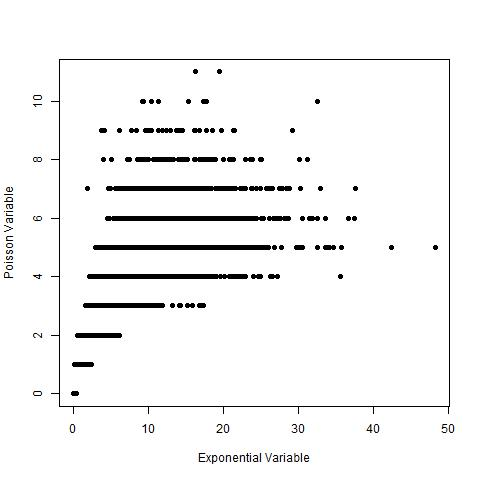
\includegraphics[width=0.9\textwidth]{Copula_model_ex}
\caption{}
\label{fig:newdist}
\end{figure}
% 
 
\trish{So what do we learn from Figure \ref{fig:newdist}? Tell us here.}

\trish{I STOPPED HERE - This is much better but still very difficult to
  follow.  You need need need a running example that is theoretically
  interesting, like the Ratcliff model (too hard, I think), or SDT.  Use
  that instead of arbitrary joint distributions.  I see the added things
  below, but without a running example they don't integrate well into the
  text.}

